\textbf{{1.死锁检测}}

{a.~}\textbf{资源分配图}

进程的死锁问题可以用有向图更加准确而形象地描述,这种有向图称为系统资源分配图。

\textbf{b. 死锁定理}

可以用简化资源分配图的方法来检测系统状态S是否是死锁状态。简化方法如下:

\textbf{首先},在资源分配图中,\textbf{找出一个既不阻塞又非孤立的进程节点Pi}。因进程Pi获得了所需要的全部资源,它能继续运行直到完成,然后释放其占有的所有资源;

\textbf{其次,}进程Pi释放资源后,可以唤醒因等待这些资源而阻塞的进程,原来阻塞的进程可能变为非阻塞进程;

\textbf{最后,}重复前两步的简化过程后,若能消去图中所有边,使所有进程成为孤立节点,则称该图是可完全简化的;若不能通过任何过程使该图完全简化,则称该图是不可完全简化的。

S为死锁状态的条件是:\textbf{{当且仅当S状态的资源分配图是不可完全简化的,该定理称为死锁定理}。}

\textbf{{2.死锁检测算法}}

(1)\textbf{基本思想是:}获得某时刻t系统中各类可利用资源的数目向量available(t),对于系统中的一组进程\{P1,P2,
,Pn\},\textbf{找出那些对各类资源请求数目均小于系统现有的各类可利用资源数目的进程}。这样的进程可以获得它们所需要的全部资源并运行结束,当运行结束后,它们会释放所占有的全部资源,从而使可用资源数目增加,将这样的进程加入到可运行结束的进程序列中,然后对剩下的进程再进行上述考查。如果一组进程中有几个不属于该序列,那么它们会发生死锁。\\
(2)与银行家算法和安全性算法类似,死锁检测算法也需要几个数据结构。\\
\textbf{a.} Available:表示当前可用资源的向量;\\
\textbf{b.} Allocation:表示已经分配的资源矩阵;\\
\textbf{c.} Request:表示进程请求资源的矩阵;\\
\textbf{d.} 临时变量:Work与Finish两个向量,其作用和安全性算法中的相同。

(3)死锁检测算法如下图所示。

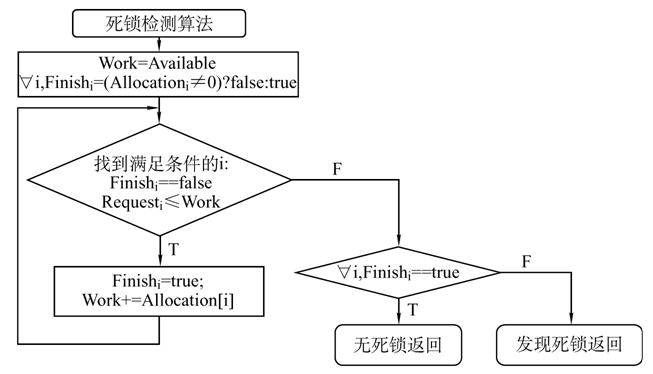
\includegraphics[width=3.33333in,height=1.90625in]{png-jpeg-pics/62353A91665DA4A4DE8E386B13D7AE31.png}

\textbf{{3.死锁解除}}

一旦检测出系统中出现了死锁,就应使陷入死锁的进程从死锁状态中解脱出来。{常用的解除死锁方法有两种:}

\textbf{a.
剥夺资源:}从其他进程中抢占足够的资源给死锁的进程以解除其死锁状态;\\
\textbf{b.
撤销进程:}撤销一些进程,直到有足够的资源分配给其他进程,解除死锁状态。
